% Options for packages loaded elsewhere
\PassOptionsToPackage{unicode}{hyperref}
\PassOptionsToPackage{hyphens}{url}
%
\documentclass[
  ignorenonframetext,
]{beamer}
\usepackage{pgfpages}
\setbeamertemplate{caption}[numbered]
\setbeamertemplate{caption label separator}{: }
\setbeamercolor{caption name}{fg=normal text.fg}
\beamertemplatenavigationsymbolsempty
% Prevent slide breaks in the middle of a paragraph
\widowpenalties 1 10000
\raggedbottom
\setbeamertemplate{part page}{
  \centering
  \begin{beamercolorbox}[sep=16pt,center]{part title}
    \usebeamerfont{part title}\insertpart\par
  \end{beamercolorbox}
}
\setbeamertemplate{section page}{
  \centering
  \begin{beamercolorbox}[sep=12pt,center]{part title}
    \usebeamerfont{section title}\insertsection\par
  \end{beamercolorbox}
}
\setbeamertemplate{subsection page}{
  \centering
  \begin{beamercolorbox}[sep=8pt,center]{part title}
    \usebeamerfont{subsection title}\insertsubsection\par
  \end{beamercolorbox}
}
\AtBeginPart{
  \frame{\partpage}
}
\AtBeginSection{
  \ifbibliography
  \else
    \frame{\sectionpage}
  \fi
}
\AtBeginSubsection{
  \frame{\subsectionpage}
}
\usepackage{lmodern}
\usepackage{amssymb,amsmath}
\usepackage{ifxetex,ifluatex}
\ifnum 0\ifxetex 1\fi\ifluatex 1\fi=0 % if pdftex
  \usepackage[T1]{fontenc}
  \usepackage[utf8]{inputenc}
  \usepackage{textcomp} % provide euro and other symbols
\else % if luatex or xetex
  \usepackage{unicode-math}
  \defaultfontfeatures{Scale=MatchLowercase}
  \defaultfontfeatures[\rmfamily]{Ligatures=TeX,Scale=1}
\fi
\usetheme[]{Antibes}
\usecolortheme{beaver}
\usefonttheme{structurebold}
% Use upquote if available, for straight quotes in verbatim environments
\IfFileExists{upquote.sty}{\usepackage{upquote}}{}
\IfFileExists{microtype.sty}{% use microtype if available
  \usepackage[]{microtype}
  \UseMicrotypeSet[protrusion]{basicmath} % disable protrusion for tt fonts
}{}
\makeatletter
\@ifundefined{KOMAClassName}{% if non-KOMA class
  \IfFileExists{parskip.sty}{%
    \usepackage{parskip}
  }{% else
    \setlength{\parindent}{0pt}
    \setlength{\parskip}{6pt plus 2pt minus 1pt}}
}{% if KOMA class
  \KOMAoptions{parskip=half}}
\makeatother
\usepackage{xcolor}
\IfFileExists{xurl.sty}{\usepackage{xurl}}{} % add URL line breaks if available
\IfFileExists{bookmark.sty}{\usepackage{bookmark}}{\usepackage{hyperref}}
\hypersetup{
  pdftitle={Séance 2.1: Analyse données digitales},
  pdfauthor={Visseho Adjiwanou, PhD.},
  hidelinks,
  pdfcreator={LaTeX via pandoc}}
\urlstyle{same} % disable monospaced font for URLs
\newif\ifbibliography
\usepackage{longtable,booktabs}
\usepackage{caption}
% Make caption package work with longtable
\makeatletter
\def\fnum@table{\tablename~\thetable}
\makeatother
\usepackage{graphicx,grffile}
\makeatletter
\def\maxwidth{\ifdim\Gin@nat@width>\linewidth\linewidth\else\Gin@nat@width\fi}
\def\maxheight{\ifdim\Gin@nat@height>\textheight\textheight\else\Gin@nat@height\fi}
\makeatother
% Scale images if necessary, so that they will not overflow the page
% margins by default, and it is still possible to overwrite the defaults
% using explicit options in \includegraphics[width, height, ...]{}
\setkeys{Gin}{width=\maxwidth,height=\maxheight,keepaspectratio}
% Set default figure placement to htbp
\makeatletter
\def\fps@figure{htbp}
\makeatother
\setlength{\emergencystretch}{3em} % prevent overfull lines
\providecommand{\tightlist}{%
  \setlength{\itemsep}{0pt}\setlength{\parskip}{0pt}}
\setcounter{secnumdepth}{-\maxdimen} % remove section numbering

\title{Séance 2.1: Analyse données digitales}
\author{Visseho Adjiwanou, PhD.}
\date{16 June 2021}
\institute{SICSS - Montréal}

\begin{document}
\frame{\titlepage}

\begin{frame}{Introduction}
\protect\hypertarget{introduction}{}

\begin{itemize}[<+->]
\tightlist
\item
  We need surveys even in the digital age.
\item
  We need surveys ---even--- especially in the digital age.
\end{itemize}

Matthews Salganik

\end{frame}

\begin{frame}{Plan de présentation}
\protect\hypertarget{plan-de-pruxe9sentation}{}

\end{frame}

\begin{frame}{Introduction}
\protect\hypertarget{introduction-1}{}

\begin{itemize}
\item
  Avec l'abondance des données digitales et digitalisées, on peut penser
  que nous n'avons plus besoin d'enquêtes
\item
  La réponse est plutôt, à cause des données digitales, nous avons plus
  que besoin d'enquêtes
\item
  Nous aurons besoin d'enquêtes pour les raisons suivantes:

  \begin{itemize}
  \tightlist
  \item
    les limites des données massives
  \item
    (internal states vs.~external states)
  \item
    inaccessibilité des données massives
  \end{itemize}
\item
  La différence va être la manière de poser les questions qui va être
  différente
\end{itemize}

\end{frame}

\begin{frame}{Évolution des enquêtes}
\protect\hypertarget{uxe9volution-des-enquuxeates}{}

\begin{longtable}[]{@{}lll@{}}
\toprule
& Échantillonnage & Interviews\tabularnewline
\midrule
\endhead
Première période & Probabiliste & Face à face\tabularnewline
\bottomrule
\end{longtable}

\end{frame}

\begin{frame}{Évolution des enquêtes}
\protect\hypertarget{uxe9volution-des-enquuxeates-1}{}

\begin{longtable}[]{@{}lll@{}}
\toprule
& Échantillonnage & Interviews\tabularnewline
\midrule
\endhead
Première période & Probabiliste & Face à face\tabularnewline
Deuxième période & Probabilité de & Téléphone\tabularnewline
& numérotation numé- &\tabularnewline
& rique aléatoire &\tabularnewline
\bottomrule
\end{longtable}

\end{frame}

\begin{frame}{Évolution des enquêtes}
\protect\hypertarget{uxe9volution-des-enquuxeates-2}{}

\begin{longtable}[]{@{}lll@{}}
\toprule
& Échantillonnage & Interviews\tabularnewline
\midrule
\endhead
Première période & Probabiliste & Face à face\tabularnewline
Deuxième période & Probabilité de & Téléphone\tabularnewline
& numérotation numé- &\tabularnewline
& rique aléatoire &\tabularnewline
Troisième période & Non probabiliste & Par ordinateur\tabularnewline
\bottomrule
\end{longtable}

\end{frame}

\begin{frame}{Évolution des enquêtes}
\protect\hypertarget{uxe9volution-des-enquuxeates-3}{}

\begin{longtable}[]{@{}llll@{}}
\toprule
& Échantillonnage & Interviews & Environnement des
données\tabularnewline
\midrule
\endhead
Première période & Probabiliste & Face à face & Autonome\tabularnewline
Deuxième période & Probabilité de & Téléphone & Autonome\tabularnewline
& numérotation numé- & &\tabularnewline
& rique aléatoire & &\tabularnewline
Troisième période & Non probabiliste & Par ordinateur &
Lié\tabularnewline
\bottomrule
\end{longtable}

\end{frame}

\hypertarget{erreurs}{%
\section{Erreurs}\label{erreurs}}

\begin{frame}{Aperçu 1:}
\protect\hypertarget{aperuxe7u-1}{}

\begin{itemize}
\tightlist
\item
  Biais et variance
\end{itemize}

\end{frame}

\begin{frame}{Aperçu 2:}
\protect\hypertarget{aperuxe7u-2}{}

\url{https://academic.oup.com/poq/article/74/5/849/1817502}

\begin{itemize}
\tightlist
\item
  Erreur totale = erreur de mesure + erreur de couverture
\end{itemize}

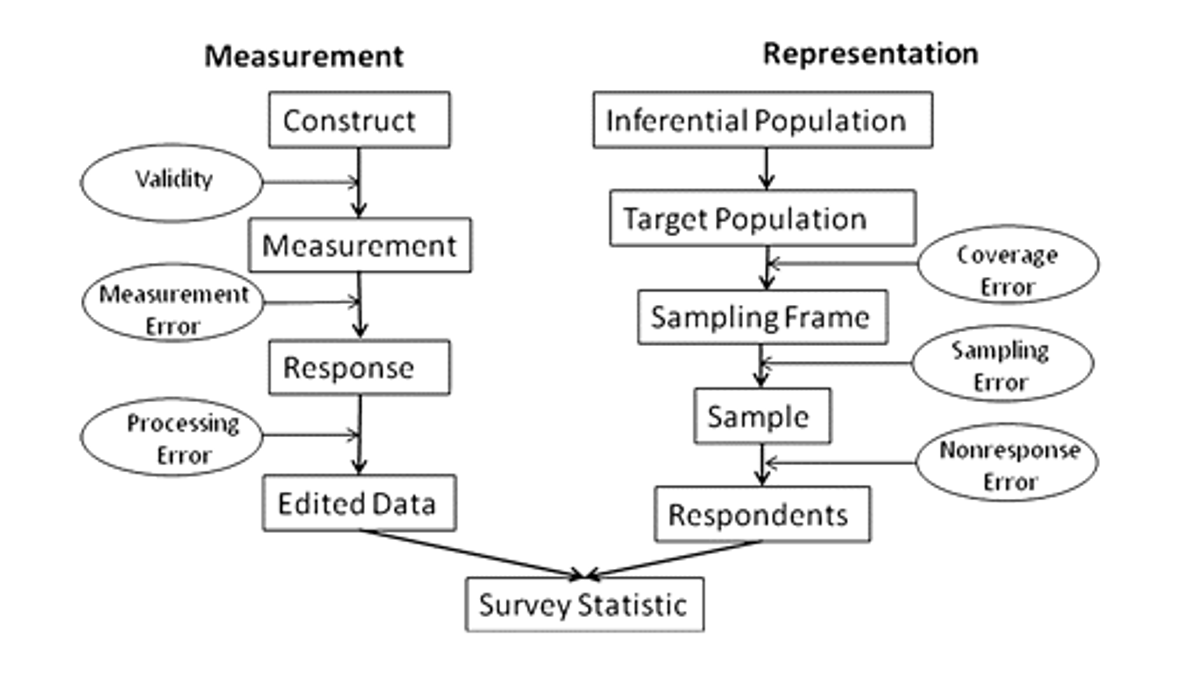
\includegraphics{../Données/enq1.png}

\begin{itemize}
\tightlist
\item
  Le cadre d'erreur totale d'enquête nous aide également à réfléchir à
  la façon dont l'ère numérique peut créer de nouvelles opportunités (à
  qui demander et comment demander)
\end{itemize}

\end{frame}

\hypertarget{uxe9chantillonnage-probabiliste-et-non-probabiliste}{%
\section{Échantillonnage probabiliste et non
probabiliste}\label{uxe9chantillonnage-probabiliste-et-non-probabiliste}}

\begin{frame}{Non probabiliste}
\protect\hypertarget{non-probabiliste}{}

\begin{longtable}[]{@{}llll@{}}
\toprule
& Échantillonnage & Interviews & Environnement des
données\tabularnewline
\midrule
\endhead
Première période & Probabiliste & Face à face & Autonome\tabularnewline
Deuxième période & Probabilité de & Téléphone & Autonome\tabularnewline
& numérotation numé- & &\tabularnewline
& rique aléatoire & &\tabularnewline
Troisième période & \textbf{Non probabiliste} & Par ordinateur &
Lié\tabularnewline
\bottomrule
\end{longtable}

\end{frame}

\begin{frame}{Échantillonnage probabiliste}
\protect\hypertarget{uxe9chantillonnage-probabiliste}{}

\begin{itemize}
\item
  Échantillon probabiliste (approximativement) : chaque unité d'une
  population de base a une probabilité d'inclusion connue et non nulle
\item
  Tous les échantillons probabilistes ne ressemblent pas à des versions
  miniatures de la population
\item
  Mais, avec une pondération appropriée, les échantillons probabilistes
  peuvent produire des estimations non biaisées de la population de base
\end{itemize}

\end{frame}

\begin{frame}{Échantillonnage probabiliste}
\protect\hypertarget{uxe9chantillonnage-probabiliste-1}{}

Principaux enseignements de l'échantillonnage probabiliste: - La façon
dont vous collectez vos données a un impact sur la façon dont vous
faites des inférences - Se concentre sur les propriétés des estimateurs
et non sur les propriétés des échantillons

\end{frame}

\begin{frame}{Principe}
\protect\hypertarget{principe}{}

\[ \hat{\bar y} = \frac{\sum y_i/\pi_i}{N} \]

\(\pi_i\) : probabilité d'inclusion de l'individu i

encore appelé - estimateur Horvitz-Thompson - estimateur \(\pi_i\)

\end{frame}

\begin{frame}[fragile]{Inférence}
\protect\hypertarget{infuxe9rence}{}

\begin{itemize}
\item
  Echantillonnage probabiliste en théorie

\begin{verbatim}
                          répondants 
\end{verbatim}

  \(\text{information connu sur l'échantillon} \Bigg\}\) estimateurs
\item
  Echantillonnage probabiliste en pratique

\begin{verbatim}
                            répondants 
\end{verbatim}

  \(\text{information estimée sur l'échantillon} \Bigg\}\) estimateurs
  Information auxilliaire + hypothèses
\item
  Echantillonnage non-probabiliste

\begin{verbatim}
                            répondants 
\end{verbatim}

  \(\text{information connu sur l'échantillon} \Bigg\}\) estimateurs
  Information auxilliaire + hypothèses
\end{itemize}

\end{frame}

\begin{frame}{Exemple}
\protect\hypertarget{exemple}{}

Imaginez que vous vouliez estimer la taille moyenne des étudiants de
l'UQAM. - Supposons que 50\% sont des hommes et 50\% sont des femmes -
Vous vous situez à l'extérieur de la Bibliothèque et recrutez un
échantillon non aléatoire de 60 étudiants de l'UQAM - Mâles (n= 20) :
Taille moyenne : 180cm - Femelles (n=40) : Taille moyenne : 170cm

Quelle est l'estimé de la taille moyenne?

\end{frame}

\begin{frame}{Exemple}
\protect\hypertarget{exemple-1}{}

\begin{itemize}
\item
  Moyenne de l'échantillon = 173.3 cm =
  \(\frac{180*20 + 170*40}{20 + 40}\)
\item
  Moyenne pondérée = 175 cm = \((180*0.5 + 170*0.5)\)
\item
  L'estimation pondérée utilise des informations auxiliaires et des
  hypothèses
\item
  Comment cela pourrait-il mal tourner ?
\end{itemize}

\end{frame}

\begin{frame}{Conclusion}
\protect\hypertarget{conclusion}{}

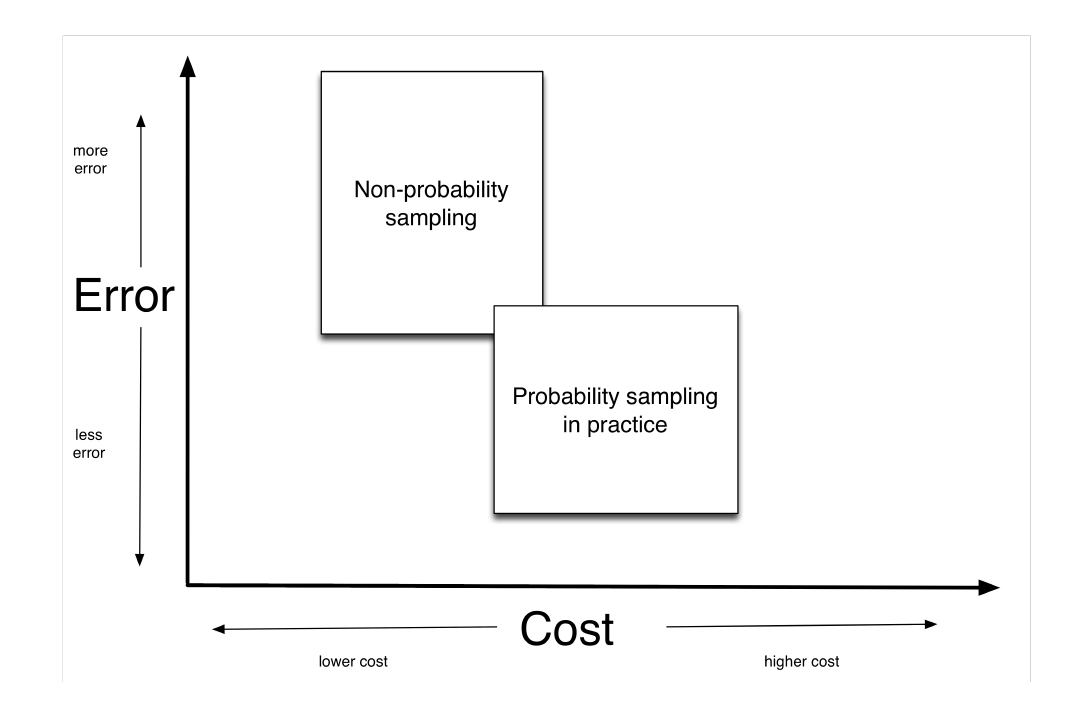
\includegraphics{../Données/enq2.png}

\end{frame}

\begin{frame}{Conclusion}
\protect\hypertarget{conclusion-1}{}

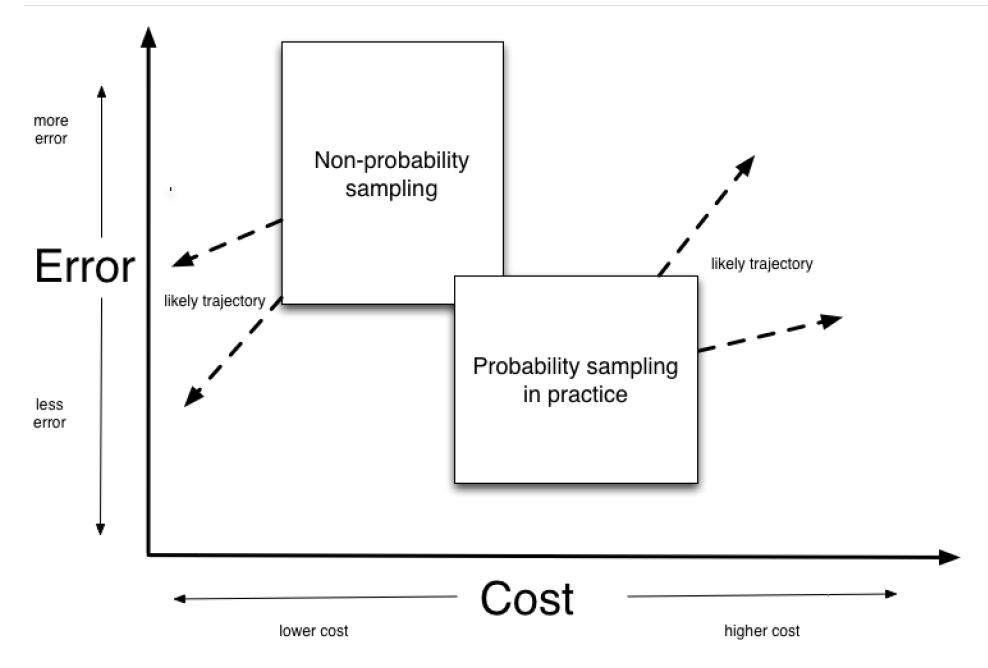
\includegraphics{../Données/enq3.png}

\end{frame}

\begin{frame}{Conclusion}
\protect\hypertarget{conclusion-2}{}

\begin{itemize}
\tightlist
\item
  Les échantillons n'ont pas besoin de ressembler à des mini-populations
\item
  La clé pour faire de bonnes estimations est que le processus
  d'estimation prenne en compte le processus d'échantillonnage
\item
  Il n'y a pas de différence nette entre l'échantillonnage probabiliste
  en pratique et l'échantillonnage non probabiliste
\item
  Pour en savoir plus : Lohr (2009) ou Sandal et al (2013)
\end{itemize}

\end{frame}

\hypertarget{enquuxeates-administruxe9es-par-les-machines}{%
\section{Enquêtes administrées par les
machines}\label{enquuxeates-administruxe9es-par-les-machines}}

\begin{frame}{Administré par ordinateur}
\protect\hypertarget{administruxe9-par-ordinateur}{}

\begin{longtable}[]{@{}llll@{}}
\toprule
& Échantillonnage & Interviews & Environnement des
données\tabularnewline
\midrule
\endhead
Première période & Probabiliste & Face à face & Autonome\tabularnewline
Deuxième période & Probabilité de & Téléphone & Autonome\tabularnewline
& numérotation numé- & &\tabularnewline
& rique aléatoire & &\tabularnewline
Troisième période & Non probabiliste & \textbf{Par ordinateur} &
Lié\tabularnewline
\bottomrule
\end{longtable}

\end{frame}

\hypertarget{combiner-les-enquuxeates-avec-les-donnuxe9es-massives}{%
\section{Combiner les enquêtes avec les données
massives}\label{combiner-les-enquuxeates-avec-les-donnuxe9es-massives}}

\begin{frame}{Lié}
\protect\hypertarget{liuxe9}{}

\begin{longtable}[]{@{}llll@{}}
\toprule
& Échantillonnage & Interviews & Environnement des
données\tabularnewline
\midrule
\endhead
Première période & Probabiliste & Face à face & Autonome\tabularnewline
Deuxième période & Probabilité de & Téléphone & Autonome\tabularnewline
& numérotation numé- & &\tabularnewline
& rique aléatoire & &\tabularnewline
Troisième période & Non probabiliste & Par ordinateur &
\textbf{Lié}\tabularnewline
\bottomrule
\end{longtable}

\end{frame}

\begin{frame}{Deux perspectives}
\protect\hypertarget{deux-perspectives}{}

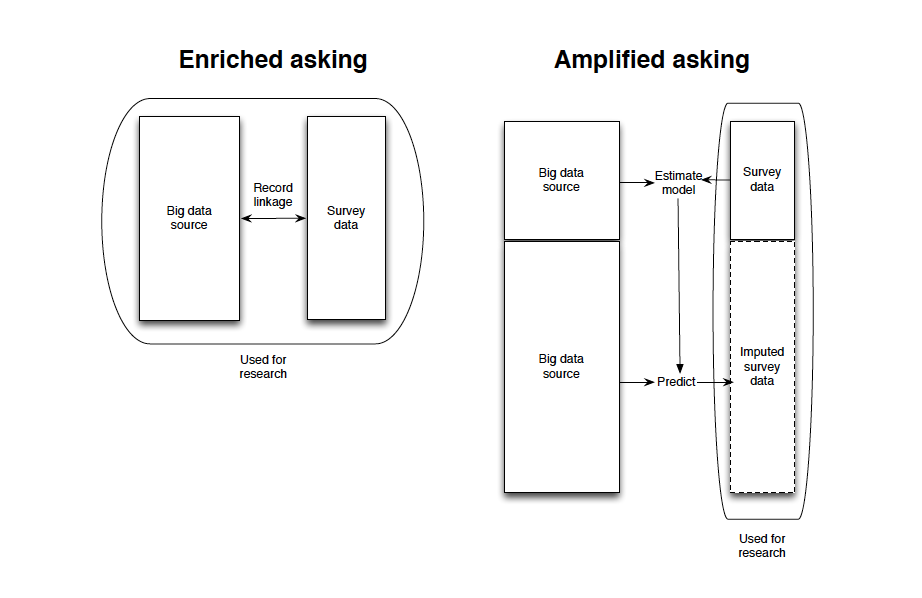
\includegraphics{../Données/enq4.png}

\end{frame}

\begin{frame}{cas 1:}
\protect\hypertarget{cas-1}{}

\href{https://www.jstor.org/stable/23359641}{Ansolabehere and Hersh
(2012)}


\includegraphics{../Données/enq5.png}

\end{frame}

\begin{frame}{Cas 2:}
\protect\hypertarget{cas-2}{}

\href{https://science.sciencemag.org/content/350/6264/1073}{Blumenstock,
Cadamuro, and On (2015)}

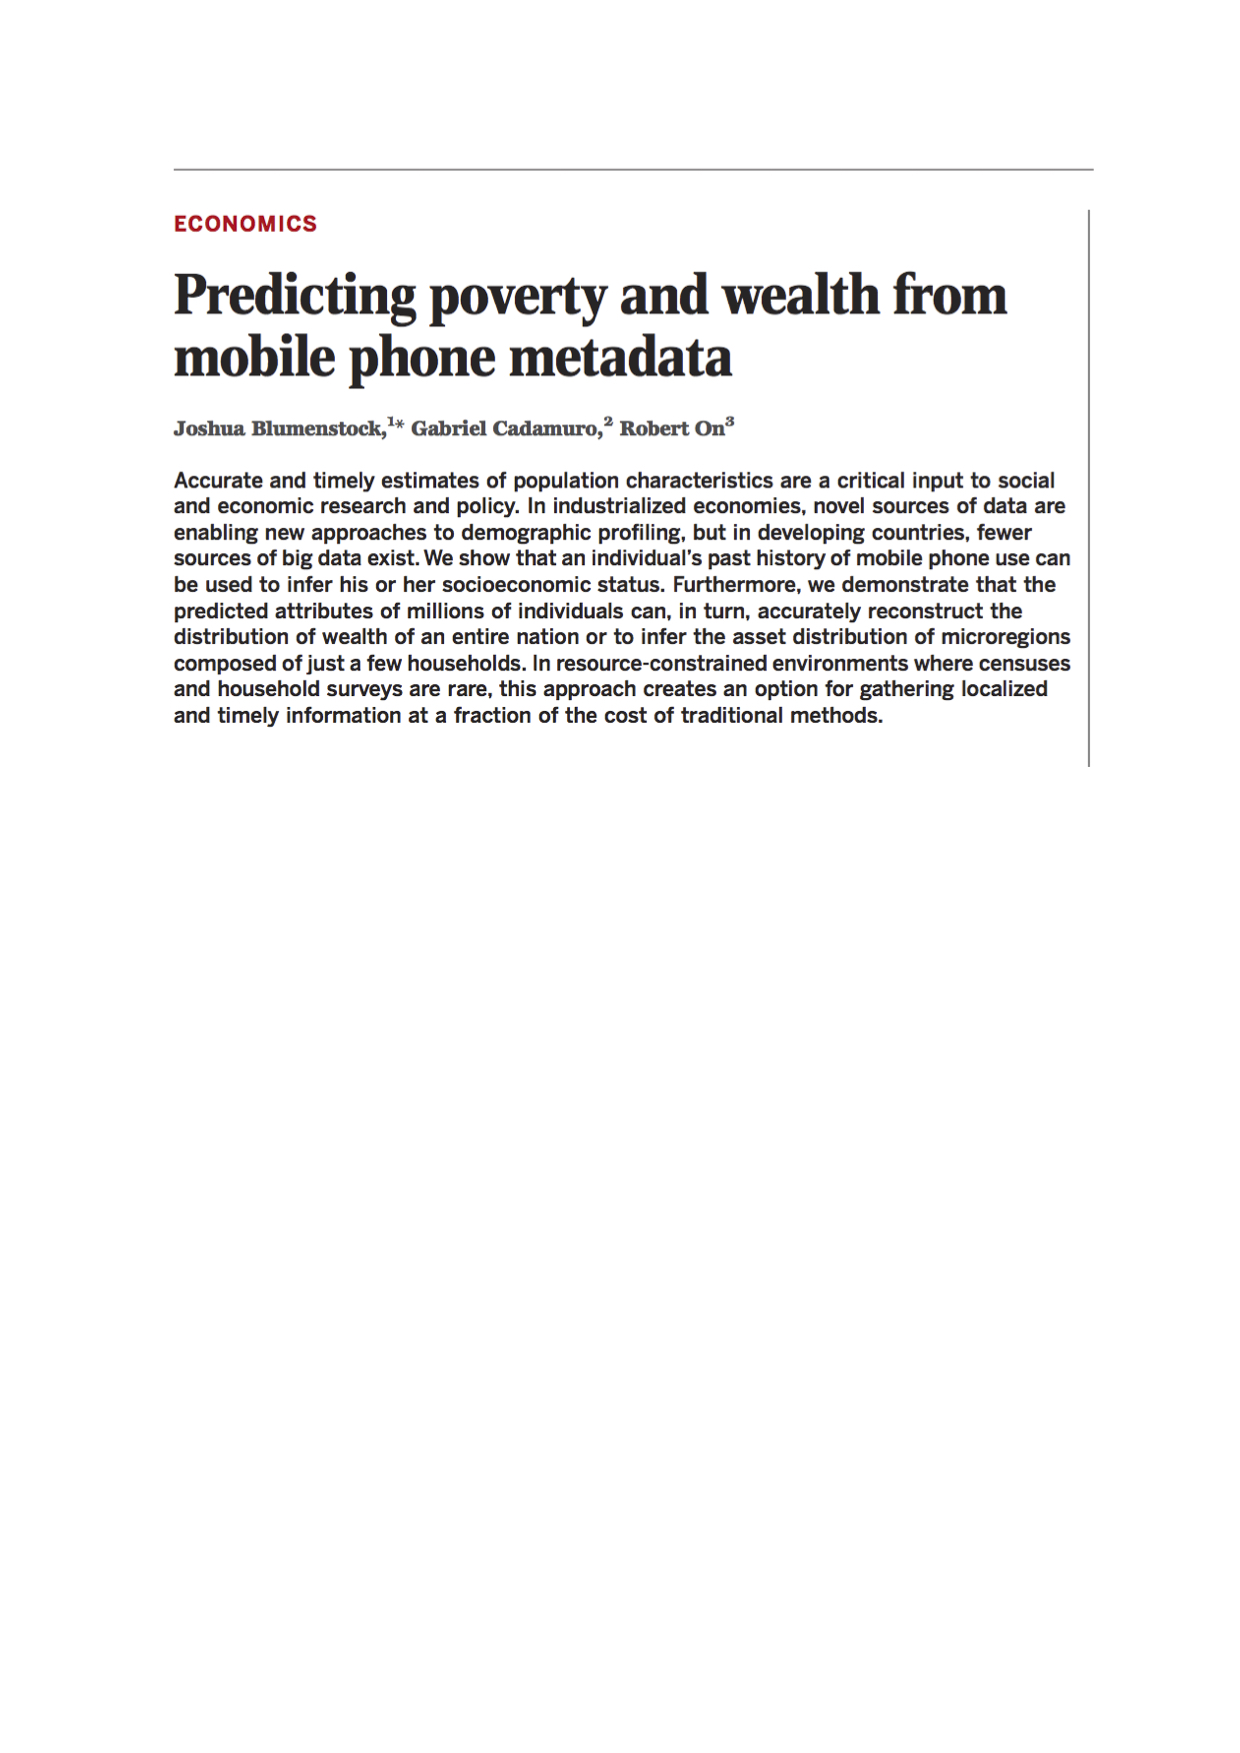
\includegraphics{../Données/Blumenstock.jpg}

\end{frame}

\begin{frame}{Prédire la pauvreté\}}
\protect\hypertarget{pruxe9dire-la-pauvretuxe9}{}

\begin{itemize}
\tightlist
\item
  Contexte: La répartition géographique de la pauvreté et de la richesse
  est utilisée pour prendre des décisions sur l'allocation des
  ressources et fournit une base pour l'étude des inégalités et des
  déterminants de la croissance économique.

  \begin{itemize}
  \tightlist
  \item
    Problèmes en ASS: Enquête clairsemée sur la pauvreté
  \end{itemize}
\end{itemize}

\end{frame}

\begin{frame}{Prédire la pauvreté\}}
\protect\hypertarget{pruxe9dire-la-pauvretuxe9-1}{}

L'étude combine des données volumineuses (Big Data) avec des données
d'enquête - Big data: base de données contenant des enregistrements de
milliards d'interactions sur le plus grand réseau de téléphonie mobile
du Rwanda auprès de 1,5 million d'individus uniques - Enquête: enquêtes
téléphoniques de suivi d'un échantillon aléatoire stratifié
géographiquement de 856 abonnés individuels - Les données de téléphonie
mobile sont utilisées par de plus en plus de personnes en Afrique
subsaharienne - Téléphones portables peuvent: - Capturer des
informations riches sur la fréquence et le calendrier des événements de
communication - Refléter la structure complexe du réseau social d'un
individu - Révéler le modèle de choix de lieu de voyage et - Histoires
de consommation et dépenses

\end{frame}

\begin{frame}{Prédire la pauvreté\}}
\protect\hypertarget{pruxe9dire-la-pauvretuxe9-2}{}

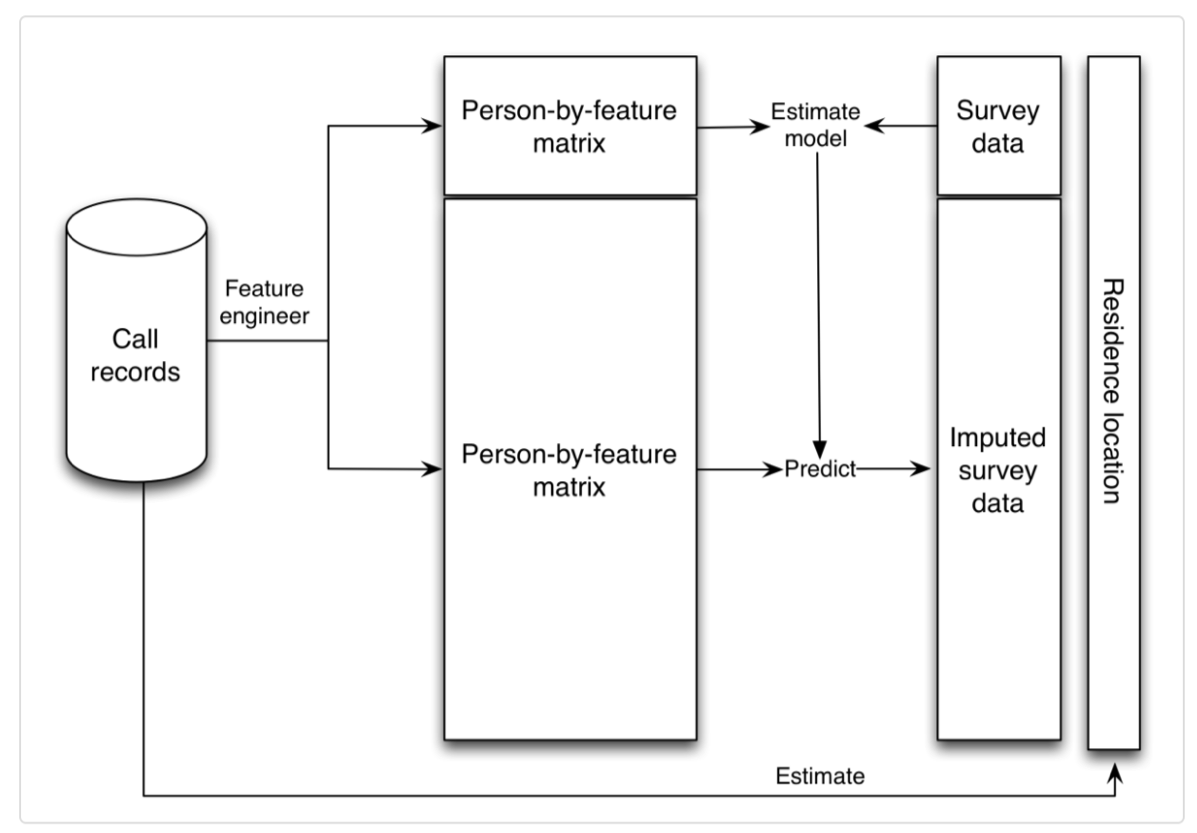
\includegraphics{../Données/Matthews2.png}

\end{frame}

\begin{frame}{Prédire la pauvreté\}}
\protect\hypertarget{pruxe9dire-la-pauvretuxe9-3}{}

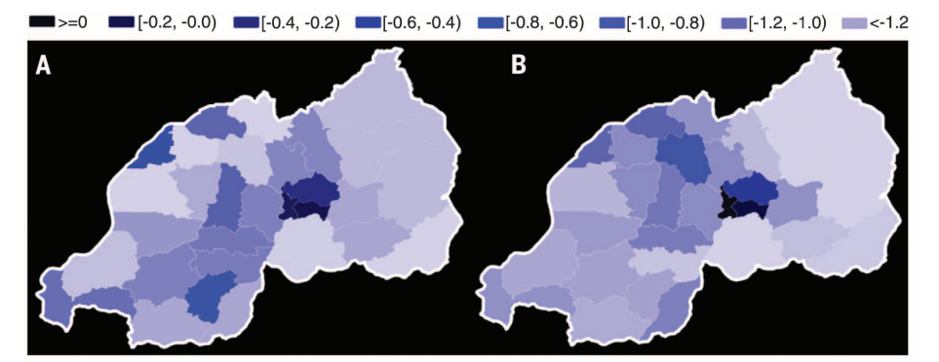
\includegraphics{../Données/blum_pp.png}

\end{frame}

\begin{frame}{Prédire la pauvreté\}}
\protect\hypertarget{pruxe9dire-la-pauvretuxe9-4}{}

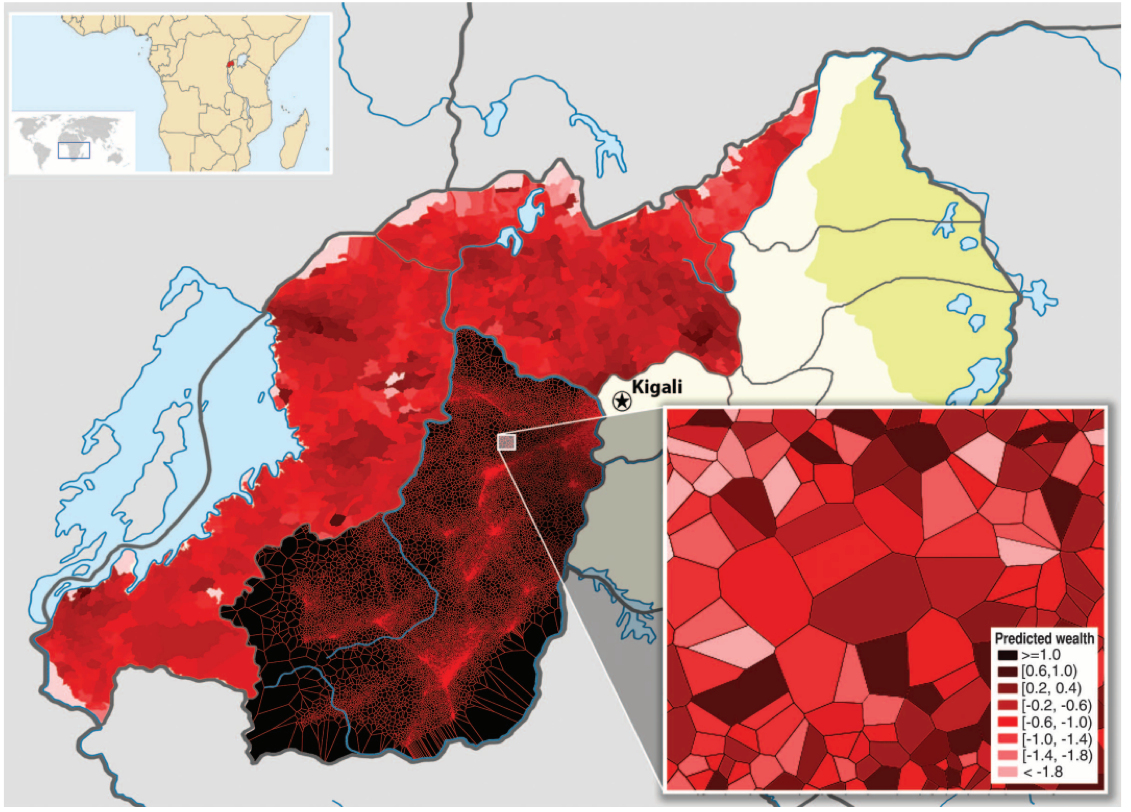
\includegraphics{../Données/blum_pp2.png}

\end{frame}

\begin{frame}{Prédire la pauvreté\}}
\protect\hypertarget{pruxe9dire-la-pauvretuxe9-5}{}

\begin{itemize}
\tightlist
\item
  Les estimations de Blumenstock et de ses collègues étaient environ 10
  fois plus rapides et 50 fois moins chères (lorsque le coût est mesuré
  en termes de coûts variables)
\item
  Cette recette ne contient que deux ingrédients et deux étapes. Les
  ingrédients sont:

  \begin{itemize}
  \tightlist
  \item
    Une source de données volumineuse qui est large mais mince
    (c'est-à-dire qu'elle a beaucoup de personnes mais pas les
    informations dont vous avez besoin sur chaque personne) et
  \end{itemize}
\item
  Une enquête étroite mais dense (c'est-à-dire qu'elle n'a que quelques
  personnes, mais qu'elle a les informations dont vous avez besoin sur
  ces personnes)
\end{itemize}

\end{frame}

\begin{frame}{Conclusion}
\protect\hypertarget{conclusion-3}{}

\begin{itemize}
\tightlist
\item
  Les sondages et les mégadonnées sont des compléments et non des
  substituts
\item
  Parfois on fait des ``demandes enrichies'' et parfois des demandes
  ``amplifiées'' (le rôle de la source de big data est di érent dans les
  deux cas)
\item
  Ressources :
  \href{https://www.bitbybitbook.com/en/1st-ed/asking-questions/}{chapitre
  3 de bit by bit}
\end{itemize}

\end{frame}

\hypertarget{additions-et-extensions}{%
\section{Additions et extensions}\label{additions-et-extensions}}

\end{document}
